% Copyright 2022 Haute école d'ingénierie et d'architecture de Fribourg
%
% Licensed under the Apache License, Version 2.0 (the "License");
% you may not use this file except in compliance with the License.
% You may obtain a copy of the License at
%
% http://www.apache.org/licenses/LICENSE-2.0
%
% Unless required by applicable law or agreed to in writing, software
% distributed under the License is distributed on an "AS IS" BASIS,
% WITHOUT WARRANTIES OR CONDITIONS OF ANY KIND, either express or implied.
% See the License for the specific language governing permissions and
% limitations under the License.

% =============================================================================
% | HES-SO//Master - Thesis project report template                           |
% |                                                                           |
% | Originally based on the EPFL template, with many adjustments             |
% =============================================================================

% Document settings
\documentclass[a4paper,11pt,fleqn]{book}
\usepackage[utf8]{inputenc}
\usepackage[T1]{fontenc} 
\usepackage[french]{babel}



% -----------------------------------------------------------------------------
% Preamble
% -----------------------------------------------------------------------------
% =============================================================================
% | Thesis metadata                                                           |
% =============================================================================

% Thesis info
\newcommand{\ThesisTitle}{Prédiction des propriétés chimiques par machine learning}
\newcommand{\ThesisSubject}{}
\newcommand{\Orientation}{Information and communication systems (ICS) }
\newcommand{\Keywords}{}
\newcommand{\Keywordsfr}{}
\newcommand{\projectVersion}{v1.1}
\newcommand{\cdcVersion}{v1.0}

% Author
\newcommand{\AuthorFirstName}{Simon }
\newcommand{\AuthorLastName}{Barras}
\newcommand{\AuthorEmail}{simon.barrasl@edu.hefr.ch}
\newcommand{\Author}{\AuthorFirstName \AuthorLastName}

% Advisor
\newcommand{\AdvisorFirstName}{Beat }
\newcommand{\AdvisorLastName}{Wolf}
\newcommand{\AdvisorSchool}{HEIA-FR}
\newcommand{\Advisor}{Prof. \AdvisorFirstName \AdvisorLastName}
\newcommand{\AdvisorTwoFirstName}{Jonathan }
\newcommand{\AdvisorTwoLastName}{Donzallaz}
\newcommand{\AdvisorTwoSchool}{HEIA-FR}
\newcommand{\AdvisorTwo}{Assis. \AdvisorTwoFirstName \AdvisorTwoLastName}

% Main expert - TODO: suppress?
\newcommand{\ExpertFirstName}{[FirstName]}
\newcommand{\ExpertLastName}{[LastName]}
\newcommand{\Expert}{\ExpertFirstName \ExpertLastName}
\newcommand{\ExpertLab}{[Lab/Company]}

% Mendant
\newcommand{\MendantInstitut}{Inst. ChemTech}
\newcommand{\MendantOneFirstName}{Roger }
\newcommand{\MendantOneLastName}{Marti}
\newcommand{\MendantOneSchool}{HEIA-FR}
\newcommand{\MendantOne}{Prof. \MendantOneFirstName \MendantOneLastName}
\newcommand{\MendantTwoFirstName}{Florence }
\newcommand{\MendantTwoLastName}{Yerly}
\newcommand{\MendantTwoSchool}{HEIA-FR}
\newcommand{\MendantTwo}{Prof. \MendantTwoFirstName \MendantTwoLastName}

% Place (for date and place)
\newcommand{\Date}{\today}
\newcommand{\Place}{Fribourg}
         % your project data
% ==================
% Template settings
% ==================

% General tools
% -------------
\usepackage{etoolbox}
\usepackage{listings}

% Page style
% ----------
\usepackage[margin=3cm, left=3.5cm, right=3.5cm, twoside=false]{geometry}
\usepackage{fancyhdr}
\setlength{\headheight}{14pt}
\renewcommand{\sectionmark}[1]{\markright{\thesection\ #1}}
\pagestyle{fancy}

% Standard pages (inside chapters)
\fancyhf{}
\renewcommand{\headrulewidth}{0.4pt}
\renewcommand{\footrulewidth}{0.4pt}
\fancyhead[R]{\bfseries \nouppercase{\rightmark}}
\fancyhead[L]{\bfseries \nouppercase{\leftmark}}
\fancyfoot[L]{\Author \space - \ThesisTitle}
\fancyfoot[R]{\thepage}

% First page of chapters
\fancypagestyle{plain}{
	\fancyhf{}
	\renewcommand{\headrulewidth}{0pt}
	\fancyfoot[L]{\Author \space - \ThesisTitle}
	\fancyfoot[R]{\thepage}
}

% Imports for external PDFs
\fancypagestyle{addpagenumbersforpdfimports}{
	\fancyhead{}
	\renewcommand{\headrulewidth}{0pt}
	\fancyfoot{}
	\fancyfoot[R]{\thepage}
}

% Use empty style for page when clearing double pages
%\def\cleartoodd{%
%	\clearpage%
%	%\ifodd\value{page}\else\mbox{}\thispagestyle{empty}\newpage\fi%
%}

%\def\clearchap{%
%	\ifodd\value{page}\else\mbox{}\thispagestyle{empty}\fi%
%}

% \cleardoublepage replaced by \cleartoodd
%\let\origdoublepage\cleardoublepage
%\renewcommand{\cleardoublepage}{%
%	\cleartoodd%
%}

% Fonts
% -----

% Helvetica (Arial used in the MSE Word template)
\usepackage{helvet}

% Math
% ----
\usepackage{amsmath}  % better math

% Floats and figures
% ------------------
\usepackage{newfloat}          % floats
\usepackage[oneside]{caption}  % captions
\usepackage{subcaption}        % subcaptions
\usepackage[section]{placeins} % allows to put float barriers

% Float captions in italics, with label in margin
%\DeclareCaptionLabelFormat{title}{#1 #2}
%\DeclareCaptionLabelFormat{hangout}{\llap{#1 #2\hspace{5mm}}}
%\captionsetup{
%	format=hang,
%	labelformat=hangout,
%	singlelinecheck=false,
%	font={it}
%}

% Caption with source for figure
% TODO: improve this to use square brackets like the normal "caption"
\newcommand*{\captionsource}[3]{%
	\caption[{#1}]{%
		#2%
		
		\textbf{Source:} #3%
	}%
}

% Tables
% ------
\usepackage{booktabs} % much better tables
\usepackage{multirow} % allows to fuse rows
\usepackage{array}    % manipulate array
\usepackage{tabularx} % better tables

% Define new tabularx column types:
%  - R: streteched right aligned
%  - C: stretched centered
%  - N: left aligned, specified space
\newcolumntype{R}{>{\raggedleft\arraybackslash}X}%
\newcolumntype{C}{>{\centering\arraybackslash}X}%
\newcolumntype{N}[1]{>{\raggedleft\arraybackslash}p{#1}}

% Set row height multiplicator to provide more breathing space
\renewcommand{\arraystretch}{1.3} 

% Bibliography
% -------------------

% Use biber, with numeric style and no sorting (citation order)
\usepackage[
backend=biber,
style=numeric,
sorting=none,
bibencoding=auto
]{biblatex}
\addbibresource{bibliography.bib}


% Tables of contents, figures, tables and listings
% ------------------------------------------------
\usepackage{tocloft}
\newlistof{listing}{lol}{List of Listings}
\setcounter{tocdepth}{1} % Depth to 'section'
\setlength{\cftfigindent}{0pt}  % remove indentation from figures in lof
\setlength{\cftfignumwidth}{1cm}
\setlength{\cfttabindent}{0pt}  % remove indentation from tables in lot
\setlength{\cfttabnumwidth}{1cm}
\setlength{\cftlistingindent}{0pt}
\setlength{\cftlistingnumwidth}{1cm}

% Mini tables of contents
% -----------------------
\usepackage{minitoc}

% no "Contents" title
\mtcsettitle{minitoc}{Contents} 

% Layout
\setlength{\mtcindent}{-0.5em}
\mtcsetoffset{minitoc}{-1em}

% Spacing above and below table
\mtcsetfeature{minitoc}{before}{\vspace{0.5cm}}
\mtcsetfeature{minitoc}{after}{\vspace{-0.25cm}}
\renewcommand{\mtifont}{\sffamily\bfseries\large}

% Colors & graphics
% -----------------
\usepackage[table]{xcolor}    % colors
\usepackage[pdftex]{graphicx} % graphics importing
\graphicspath{{02-main/figures/}}
\definecolor{gray80}{gray}{0.80}


% Code and syntax highlighting
% ----------------------------
\usepackage[newfloat]{minted}   % code highlighting

% Typography
% ----------
\usepackage{csquotes}                    % paragraph indentation and spacing
\usepackage[defaultlines=3,all]{nowidow} % avoid widows and orphans
\usepackage{microtype}                   % typographic improvements
\usepackage{parskip}                     % No indent and auto-space between paragraphs
\usepackage[super]{nth}

\usepackage{paralist}
\usepackage{enumitem}
\setlist{after=\vspace{\baselineskip}}

% Section and chapters headings
% -----------------------------
\usepackage[explicit]{titlesec} % titles formatting
%\usepackage{titletoc} % titles formatting in ToC etc
%\usepackage{sectsty}  % sectioning commands

% -- Chapters --
% Remove "Chapter N" and use a sans-serif font

% Set layout lengths
\setlength{\headheight}{8mm}
\setlength{\footskip}{1.5cm}
\addtolength{\textheight}{-.5cm}

\titlespacing{\chapter}{-5mm}{-10mm}{3mm}
\titlespacing{\section}{-5mm}{3mm}{2mm}
\titlespacing{\subsection}{-5mm}{2mm}{2mm}
\titlespacing{\subsubsection}{-5mm}{2mm}{1mm}


%\titleformat{\chapter}[block]
%{\Huge}
%{\thechapter\hspace{12pt}\textcolor{gray80}{|}\hspace{12pt}}
%{0pt}
%{\Huge\bfseries}

\titleformat{\chapter}{\Huge\bfseries}{\llap{\thechapter\hspace{12pt}\textcolor{gray80}{|}}}{0mm}{%
	\hfill\begin{minipage}[t]{\dimexpr\textwidth}\raggedright#1\end{minipage}%
}
\titleformat{\section}{\Large\bfseries}{\llap{\thesection}}{0mm}{%
	\hfill\begin{minipage}[t]{\dimexpr\textwidth}\raggedright#1\end{minipage}%
}
\titleformat{\subsection}{\large \bfseries}{\llap{\thesubsection}}{0mm}{%
	\hfill\begin{minipage}[t]{\dimexpr\textwidth}\raggedright#1\end{minipage}%
}
\titleformat{\subsubsection}{\bfseries}{\llap{\thesubsubsection}}{0mm}{%
	\hfill\begin{minipage}[t]{\dimexpr\textwidth}\raggedright#1\end{minipage}%
}

% Misc
% ------
\usepackage{lipsum}    % filler text
\usepackage{blindtext} % random text
\usepackage{lscape}    % easy landscape pages
\usepackage{pdflscape} % landscape pages for PDFs

% Allow email typesetting
\newcommand{\email}[1]{%
	\href{mailto:#1}{\textit{#1}}%
}

% References
% -----------
\usepackage{url}

% pdf metadata
\usepackage[
	pdfauthor={\Author},
	pdftitle={\ThesisTitle},
	pdfsubject={\ThesisSubject},
	pdfkeywords={\Keywords}
	pdfduplex=DuplexFlipLongEdge]{hyperref}
		
% Hyperlinks
\hypersetup{
	colorlinks=true,
	linkcolor=black,
	citecolor=black,
	filecolor=black,
	urlcolor=black,
}
\providecommand*{\listingautorefname}{Listing}


% % Glossary
% % --------
%\usepackage[xindy,toc, nonumberlist]{glossaries}
\usepackage[acronym]{glossaries}
\makeglossaries
% Terms
% -----
% format:  \newglossaryentry{<label>}{<settings>}
% example: \newglossaryentry{computer}
%{
%	name=computer,
%	description={is a programmable machine that receives input,
%		stores and manipulates data, and provides
%		output in a useful format}
%}

\newglossaryentry{latex}
{
    name=latex,
    description={Is a markup language specially suited 
    for scientific documents}
}

% Acronyms
% --------
% format:  \newacronym{<label>}{<abbrv>}{<full>}
% example: \newacronym{lvm}{LVM}{Logical Volume Manager}
% plural:  \newacronym[longplural={Frames per Second}]{fpsLabel}{FPS}{Frame per Second}

    % template settings
% ===========================================
% = Codestyles for minted syntax highlighting
% ===========================================


% How to use (replace 'java' with language name):
% - code blocks:
%     \begin{javacode}
%     CODE
%     \end{javacode}
% - files:
%     full: \javafile{PATH}
%     extract: \javafile[startline=x, endline=y]{PATH}

% c#
\newminted{csharp}{frame=single, framesep=6pt, breaklines=true, fontsize=\scriptsize}
\newmintedfile{csharp}{frame=single, framesep=6pt, breaklines=true, 
fontsize=\scriptsize}

% Java
\newminted{java}{frame=single, framesep=6pt, breaklines=true, fontsize=\scriptsize}
\newmintedfile{java}{frame=single, framesep=6pt, breaklines=true, 
fontsize=\scriptsize}

% JavaScript
\newminted{js}{frame=single, framesep=6pt, breaklines=true, fontsize=\scriptsize}
\newmintedfile{js}{frame=single, framesep=6pt, breaklines=true, fontsize=\scriptsize}

% Scala
\newminted{scala}{frame=single, framesep=6pt, breaklines=true, fontsize=\scriptsize}
\newmintedfile{scala}{frame=single, framesep=6pt, breaklines=true, 
	fontsize=\scriptsize}

% Clojure
\newminted{clojure}{frame=single, framesep=6pt, breaklines=true, fontsize=\scriptsize}
\newmintedfile{clojure}{frame=single, framesep=6pt, breaklines=true, 
	fontsize=\scriptsize}

% Python
\newminted{python}{frame=single, framesep=6pt, breaklines=true, fontsize=\scriptsize}
\newmintedfile{python}{frame=single, framesep=6pt, breaklines=true, fontsize=\scriptsize}

% Sql
\newminted{sql}{frame=single, framesep=6pt, breaklines=true, fontsize=\scriptsize}
\newmintedfile{sql}{frame=single, framesep=6pt, breaklines=true, fontsize=\scriptsize}

% Json
\newminted{json}{frame=single, framesep=6pt, breaklines=true, fontsize=\scriptsize}
\newmintedfile{json}{frame=single, framesep=6pt, breaklines=true, 
	fontsize=\scriptsize}

% Yaml
\newminted{yaml}{frame=single, framesep=6pt, breaklines=true, 
fontsize=\scriptsize}
\newmintedfile{yaml}{frame=single, framesep=6pt, breaklines=true, 
	fontsize=\scriptsize}

% Plain text
\newminted{text}{frame=single, framesep=6pt, breaklines=true, breakanywhere, fontsize=\scriptsize}
\newmintedfile{text}{frame=single, framesep=6pt, breaklines=true, breakanywhere, fontsize=\scriptsize}       % code styles for minted
% ========================
% = TODO: Document
% ========================

% Marc's font stack
\usepackage{cmbright}       % Sans serif
\usepackage{sourcecodepro}  % Monospace
\usepackage{float}
\renewcommand{\familydefault}{\sfdefault}
  % your custom packages etc

% Glossary
% --------

% \usepackage[toc]{glossaries}
% \makeglossaries
% % Terms
% -----
% format:  \newglossaryentry{<label>}{<settings>}
% example: \newglossaryentry{computer}
%{
%	name=computer,
%	description={is a programmable machine that receives input,
%		stores and manipulates data, and provides
%		output in a useful format}
%}

\newglossaryentry{latex}
{
    name=latex,
    description={Is a markup language specially suited 
    for scientific documents}
}

% Acronyms
% --------
% format:  \newacronym{<label>}{<abbrv>}{<full>}
% example: \newacronym{lvm}{LVM}{Logical Volume Manager}
% plural:  \newacronym[longplural={Frames per Second}]{fpsLabel}{FPS}{Frame per Second}


\begin{document}


% -----------------------------------------------------------------------------
% Front matter
% -----------------------------------------------------------------------------
\frontmatter

\dominitoc

% ==========================================================================
% = HES-SO Master thesis title page (modeled after Word template, 2016-2017)
% ==========================================================================

\begin{titlepage}
\newgeometry{margin=2cm}
{\fontfamily{phv}\fontseries{mc}\selectfont
    \begin{center}
	    
\includegraphics[width=0.95\textwidth]{img/heiafr_logo}
		~\\[1.5cm]
		% Title
		{
			\Huge
			PS5 - \ThesisTitle\\Cahier des charges \\[0.5cm]
			\large Informatique et Système de Communication (ISC), 2022-2023\\[2cm]
		}
		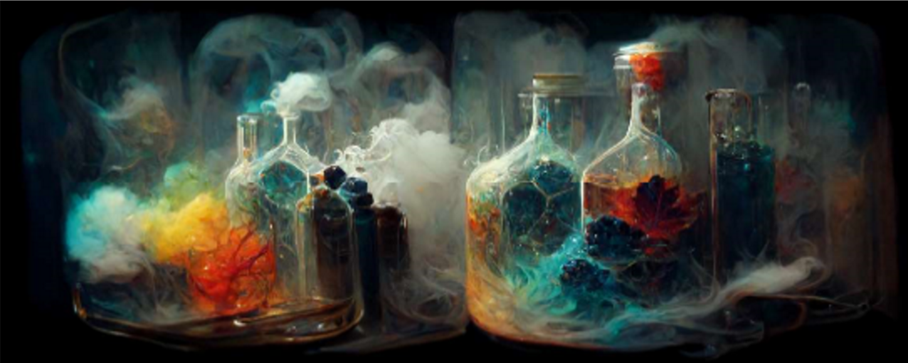
\includegraphics[width=0.8\textwidth]{img/logo.png}
		~\\[2cm]
		% Info
		{
			\begin{center}
			\begin{tabularx}{\textwidth} { %tableau pour créer 2 colonnes 
				>{\raggedright\arraybackslash}X 
				>{\raggedright\arraybackslash}X  }
					 \textbf{Etudiant} & \Author\\
					 & \\
					 \textbf{Enseignants responsables} & \Advisor \space - \AdvisorSchool \\ & \AdvisorTwo \space - \AdvisorTwoSchool \\
					 & \\
					 \textbf{Mendant} & \MendantInstitut \\ & \MendantOne \space - \MendantOneSchool \\ & \MendantTwo \space - \MendantTwoSchool\\
			\end{tabularx}
			\end{center}
			~\\[1.5cm]
		}
%		{
%			\large
%			External expert: \\
%			\Expert
%		}

        % {
        % Le code de ce projet est disponible en open source avec l'accord de tous ses
        % participants.
        % }
		\vfill
		
		 
		
		% Bottom of the page
	    {\cdcVersion}\\
		{\large \Place, HEIA-FR, \Date}
		
	\end{center}
}
\restoregeometry
\end{titlepage}






% Page for student info and signatures
% \cleardoublepage
% \chapter*{Information about this report}

\vspace{\fill}

\textbf{Contact information}

\begin{tabularx}{\textwidth}{N{2.5cm}X}
	Author:	 & \AuthorFirstName \AuthorLastName \\
	& MSE Student \\
	& HES-SO//Master \\
	& Switzerland \\
	Email: & \email{\AuthorEmail}
\end{tabularx}

\vspace{\fill}

\textbf{Declaration of honor}

{\renewcommand{\arraystretch}{2}
\begin{tabularx}{\textwidth}{N{2.5cm}X}
	& I, undersigned, \Author, hereby declare that the work submitted is 
	the result of a personal work. I certify that I have not resorted to 
	plagiarism or other forms of fraud. All sources of information used and the 
	author quotes were clearly mentioned. \\
	Place, date: & \underline{\hspace{7cm}} \\ 
	Signature: & \underline{\hspace{7cm}}
\end{tabularx}
}

\vspace{\fill}

%\textbf{Validation}

%Accepted by the HES-SO//Master (Switzerland, Lausanne) on a proposal from:
Accepté par la HES SO//Master (Suisse, Lausanne) sur proposition de

\vspace{0.5cm}

\Advisor %, Thesis project advisor

%\Expert, \ExpertLab, Main expert

\vspace{1cm}

Lieu, date: \underline{\hspace{8cm}}

\vspace{3cm}

{ \renewcommand{\arraystretch}{1.5}
\begin{tabularx}{\textwidth}{X X}
	\Advisor  & \Dean\\ 
	Advisor   & Dean, HES-SO//Master\\
\end{tabularx}
}

% Acknowledgments (your dedication etc)
% \cleardoublepage
% \chapter*{Acknowledgments}
\markboth{Acknowledgements}{Acknowledgements}
\addcontentsline{toc}{chapter}{Acknowledgements}

% -- Your text goes here --
\lipsum[1-2]
 


% Preface (to be written by someone else)
% \cleardoublepage
% \chapter*{Preface}
\markboth{Preface}{Preface}
\addcontentsline{toc}{chapter}{Preface}
% put your text here
A preface is not mandatory. It would typically be written by some other person (eg your thesis director).

\lipsum[1-2]

\bigskip
 
\noindent\textit{Lausanne, 12 Mars 2011}
\hfill T.~D.


% French + English abstracts
%\cleardoublepage
%% English abstract
\chapter*{Abstract}
%\markboth{Abstract}{Abstract}
\addcontentsline{toc}{chapter}{Abstract} % adds an entry to the table of contents

\vskip0.5cm
\textbf{Key words: } 
\Keywords


% French abstract
% \cleardoublepage
% \begin{otherlanguage}{french}
% \chapter*{Résumé}
% %\markboth{Résumé}{Résumé}

% \lipsum[1-2]

% \vskip0.5cm
% \textbf{Mots clés:} 
% \Keywordsfr
% \end{otherlanguage}



% Table of contents
\phantomsection
\chapter{Historique des versions}
\label{chap:versions}

\begin{tabular}{|m{0.15\textwidth}|m{0.7\textwidth}|m{0.15\textwidth}|} 
 \hline
 \textbf{Version} & \textbf{Changements} & \textbf{Date} \\ [0.5ex] 
 \hline
 0.1 & Document créé sur Microsoft Word avec les chapitres contexte et objectifs & 05.09.2022  \\ 
 \hline
 0.2 & Migration du document sur LaTeX et rajout de la première version du chapitre Activités & 9.10.2022  \\
 \hline
 0.3 & Finalisation du premier rendu du rapport & 10.10.2022  \\
 \hline
 1 & Version finale du cahier des charges. Les problèmes de pages blanches et de glossaire ont été réglés. De plus, le planning a été mis à jour. & 14.10.2022  \\
 \hline
\end{tabular}
\addcontentsline{toc}{chapter}{Table des matières}
\tableofcontents

% List of tables
% \cleardoublepage
% \phantomsection
% \addcontentsline{toc}{chapter}{Liste des tables}
% \listoftables

% List of listings
% \cleardoublepage
% \phantomsection
% \addcontentsline{toc}{chapter}{List of Listings}
% \listoflistings

% Restore paragraphs
\setlength{\parskip}{1em}

% Bold fonts for sections in minitoc
\renewcommand{\cftsecfont}{\sffamily\bfseries}
\renewcommand{\cftsecleader}{\sffamily\bfseries\cftdotfill{\cftdotsep}}
\renewcommand{\cftsecpagefont}{\sffamily\bfseries}


% -----------------------------------------------------------------------------
% Main matter
% -----------------------------------------------------------------------------
\mainmatter

% Chapters
\setcounter{mtc}{4} % Help minitoc skip the front matter chapters
\chapter{Contexte}
\label{chap:contexte}

Les liquides ioniques sont des éléments beaucoup utilisés en chimie. Ils permettent notamment de stocker de l'énergie mais disposent aussi de nombreuses autres applications.

Les liaisons ioniques s'obtiennent par l'attraction de deux ions de charge opposée. Les ions de charges positives et négatives sont respectivement appelés : cation et anion. Généralement, les cations sont métalliques tandis que les anions ne le sont pas. Un ion est composé d'un ou plusieurs atomes chargés électriquement.

Les possibilités de liaisons sont probablement infinies et leurs propriétés diffèrent pour chaque composition. Dans notre cas, la particularité qui nous intéresse est le point d'ébullition. Si on voulait obtenir cette information par expérience, il faudrait compter en jour le temps et les ressources consommées seraient importantes. L'objectif de ce travail de semestre est d'estimer la température d'ébullition d'un liquide ionique afin de concentrer le temps et les ressources de l'institut ChemTech de la HEIA-FR sur des liaisons validées par l'outil au préalable.

Ce travail sera utilisé comme outil de base pour un projet visant à stocker ou récupérer de l'énergie dans les phases de changements d'états d'un liquide ionique. Le but est d'y insérer en entrée le \acrfull{smiles} de l'anion et du cation et on obtiendra la température estimée.

L'écriture \acrshort{smiles} est utilisée en chimie pour décrire des molécules. Cette écriture permet de reconstruire le modèle 3D ou 2D comme ci-dessous :
\begin{center}
   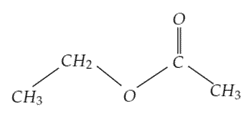
\includegraphics[height=20mm]{img/smiles_example.png}
   \captionof{figure}{Exemple de \acrshort{smiles}}
\end{center}

 
Il existe une librairie python qui permet de récupérer les informations issues d'un \acrshort{smiles}.

Ce projet a déjà été amorcé par Mme Yerly et un étudiant réalisant master de mathématiques à la HEIA-FR. Ils ont réussi à reproduire les résultats obtenus dans une étude à l'aide de la base de données fournie par cette dernière et vérifier par la base de données de l'école. Ce modèle était basé sur l'algorithme SVM (Support Vector Machine).

Ces algorithmes ont besoin de données d'entrées et de cibles. Son but sera de faire le lien entre les différents paramètres insérés et la cible la plus probable.

Dans un second temps, on pourrait aussi imaginer améliorer l'outil en rajoutant une surcouche qui déterminera le meilleur liquide ionique pour un objectif donné ou la possibilité de prédire d'autres propriétés.

\chapter{Objectifs}
\label{chap:objectifs}

Les objectifs listent les différents délivrables du projet et les principaux se retrouveront dans la liste des milestones.

\section{Principaux}
\begin{itemize}
   \item Créer une base de données regroupant les sources de données déjà utilisées et normalisées pour l'apprentissage
   \item Reproduire les résultats du projet de Mme Yerly en utilisant les mêmes technologies
   \item Créer un nouveau modèle en utilisant les données extraites des \acrshort{smiles}
\end{itemize}
\section{Secondaires}
\begin{itemize}
   \item Définir l'algorithme de machine Learning le plus efficace pour cette tâche
   \item Améliorer la base de données
   \item Améliorer l'expérience utilisateur
\end{itemize}

\include{04-cahier-des-charges/ch3_activités}
\chapter{Planning}
\label{chap:planning}

Pour faire le planning, j'ai décidé de l'intégrer le plus possible à Gitlab. En effet, j'ai choisi d'utiliser les épics, les issues et les milestones disponibles directement sur Gitlab.
Les avantages sont que le planing est très bien intégré et qu'on peut récupérer l'historique précis des actions effectuées pour compléter la tâche.
En revanche, le diagramme de Gantt n'est pas pratique à utiliser et le point de vue est orienté sur les tâches et non sur le timing.

Pour organiser le travail, j'ai choisi d'utiliser deux niveaux d'épics. Le premier représente les objectifs principaux, ceux-ci sont complétés par des sous épics qui sont les tâches à effectuer.
Ce deuxième niveau est complété par des issues qui sont les étapes à cocher pour compléter une tâche. Sur ces issues, on indiquera le poids afin de pouvoir quantifier l'effort nécessaire à la réalisation et on pourra lier des merge requests pour garder une trace des modifications.
Les milestones sont là pour rappeler les échances de différents rendus.

Le planning est directement accessible dans le menu "Roadmap" du groupe Gitlab (\href{https://gitlab.forge.hefr.ch/groups/ps5-2223-fusionprediction/-/roadmap}{lien}).

\begin{center}
    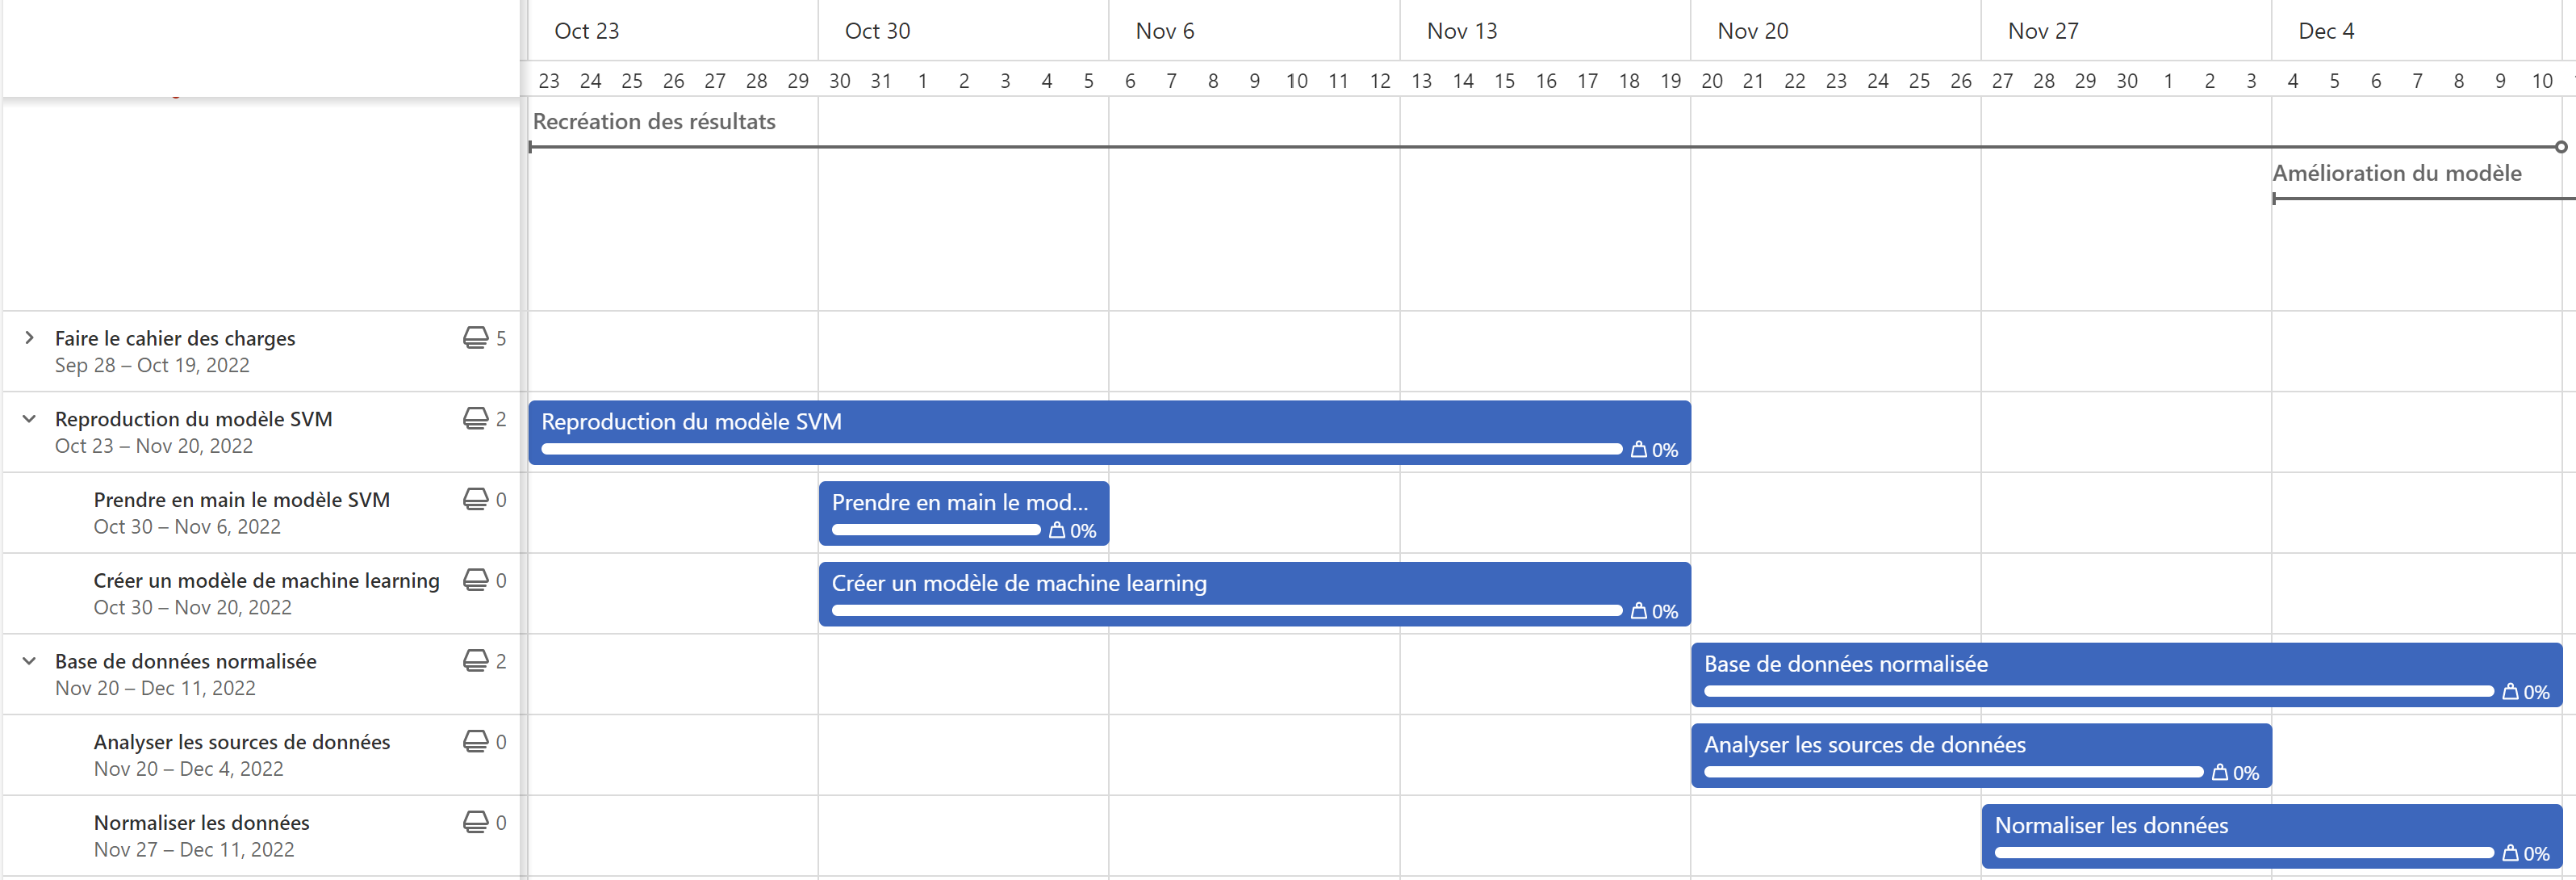
\includegraphics[width=14cm]{img/planning_1.png}
    \captionof{figure}{Planning de la recréation des résultats}
\end{center}

Ce premier planning représente la milestone qui correspond à la recréation des résultats. Il est composé de 2 épics principaux qui sont la base de données et le développement du premier modèle d'intelligence artificielle.

\begin{center}
    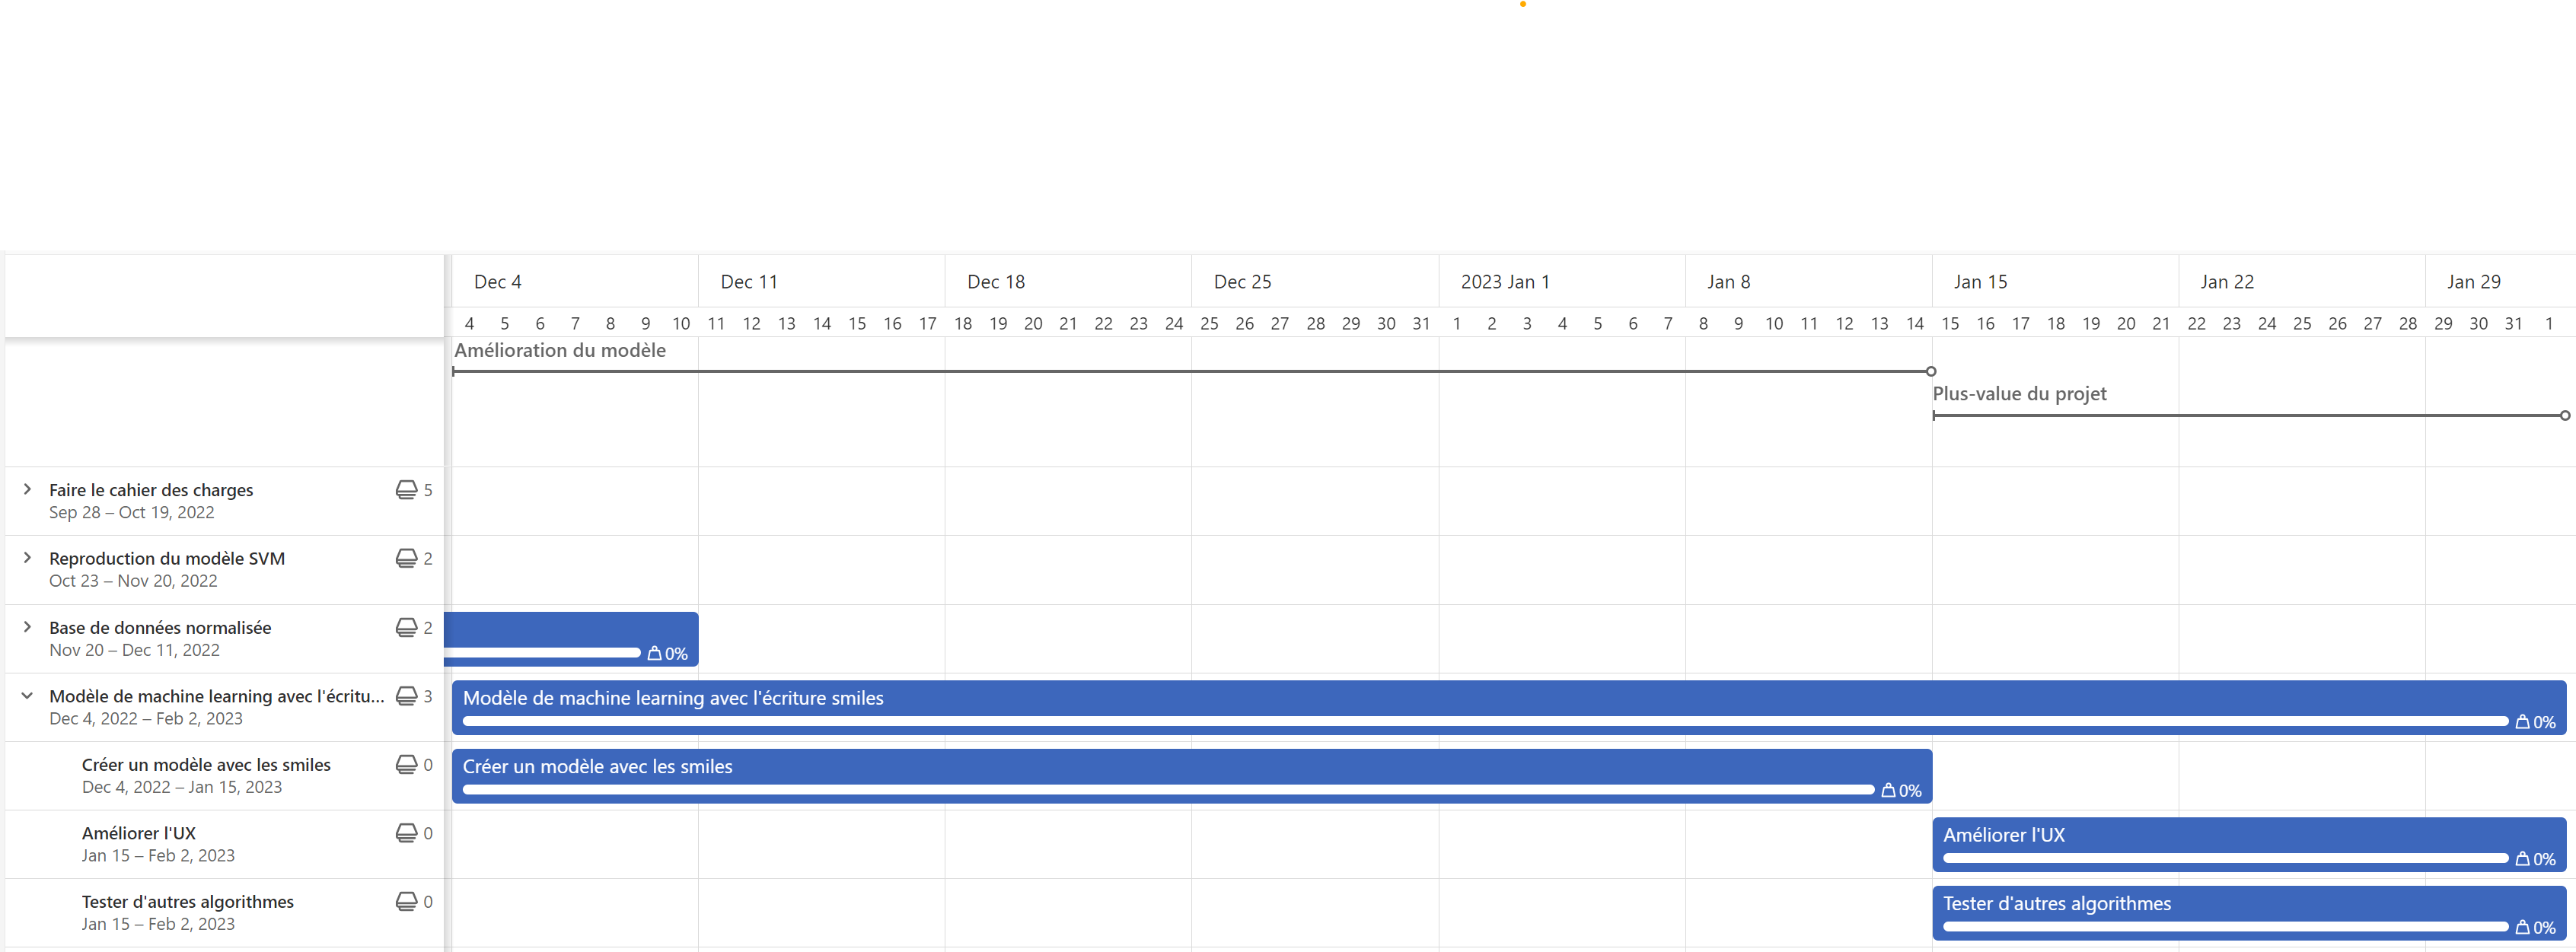
\includegraphics[width=14cm]{img/planning_2.png}
    \captionof{figure}{Planning de l'amélioration du modèle}
\end{center}

Cette deuxième partie de planing met en avant l'amélioration du modèle de machine learning à l'aide de l'écriture \acrshort{smiles}.
Elle est coupée par une milestone qui correspoond à la décision qui sera prise pour la finalisation du projet. En cas de résultats satisfaisants, nous nous concentrons sur les améliorations de l'expérience utilisateur avec une \acrshort{api}, une interface graphique ou autre solution.
Dans le cas contraire, nous pourrons essayer d'autres algorithmes afin d'améiorer les résultats de la prédiction.

% Appendices
% \appendix

% -----------------------------------------------------------------------------
% Back matter
% -----------------------------------------------------------------------------
% \backmatter

% List of figures
%\cleardoublepage
\phantomsection
\addcontentsline{toc}{chapter}{Table des figures}
\listoffigures

% Bibliography
%\cleardoublepage
%\printbibliography[title={References}, heading=bibintoc]

% Glossary
\glsaddall
\printglossary[type=\acronymtype]
% TODO: Add index

% Add your CV here if you want

\end{document}

